%!TEX program = xelatex
\documentclass[cn,hazy,pku,12pt,normal,math=newtx,cite=super]{elegantnote}
\title{溶液表面吸附的测定}

\author{刘松瑞 \quad 2100011819 \\ 组号:24 \quad 组内编号:5}
\institute{化学与分子工程学院}

\expdate{\zhdate{2023/10/11}}
\temperature{21.2 \si{^{\circ}C}}
\pressure{101.49 \si{kPa}}

\usepackage{gensymb}
\usepackage{array}
\usepackage{subfigure}
\usepackage[fontset=windows]{ctex}
\usepackage{graphicx}
\usepackage{float}
\usepackage{caption}
\usepackage{multirow}
%\usepackage{subfig}
%\usepackage{float}
\begin{document}

\maketitle

\keywords{表面吸附\quad表面张力\quad正丁醇\quad最大气泡压力法\quad吊片法}

\abstracts{
    
本次实验使用最大气泡压力法与吊片法,测量了纯水以及不同浓度的正丁醇溶液的表面张力大小
并通过实验数据,求得两种方法的水的饱和吸附量,并对计算进行误差分析。
再计算两种方法下吸附分子的横截面积,并对高浓度下考虑溶质分子的横截面积进行计算。

}

\newpage


\section{引言}

\subsection{实验目的、原理}

实验目的、原理详见预习报告图~\ref{1}。 \cite{pcl2002}

\begin{figure}[htbp]
    \centering
    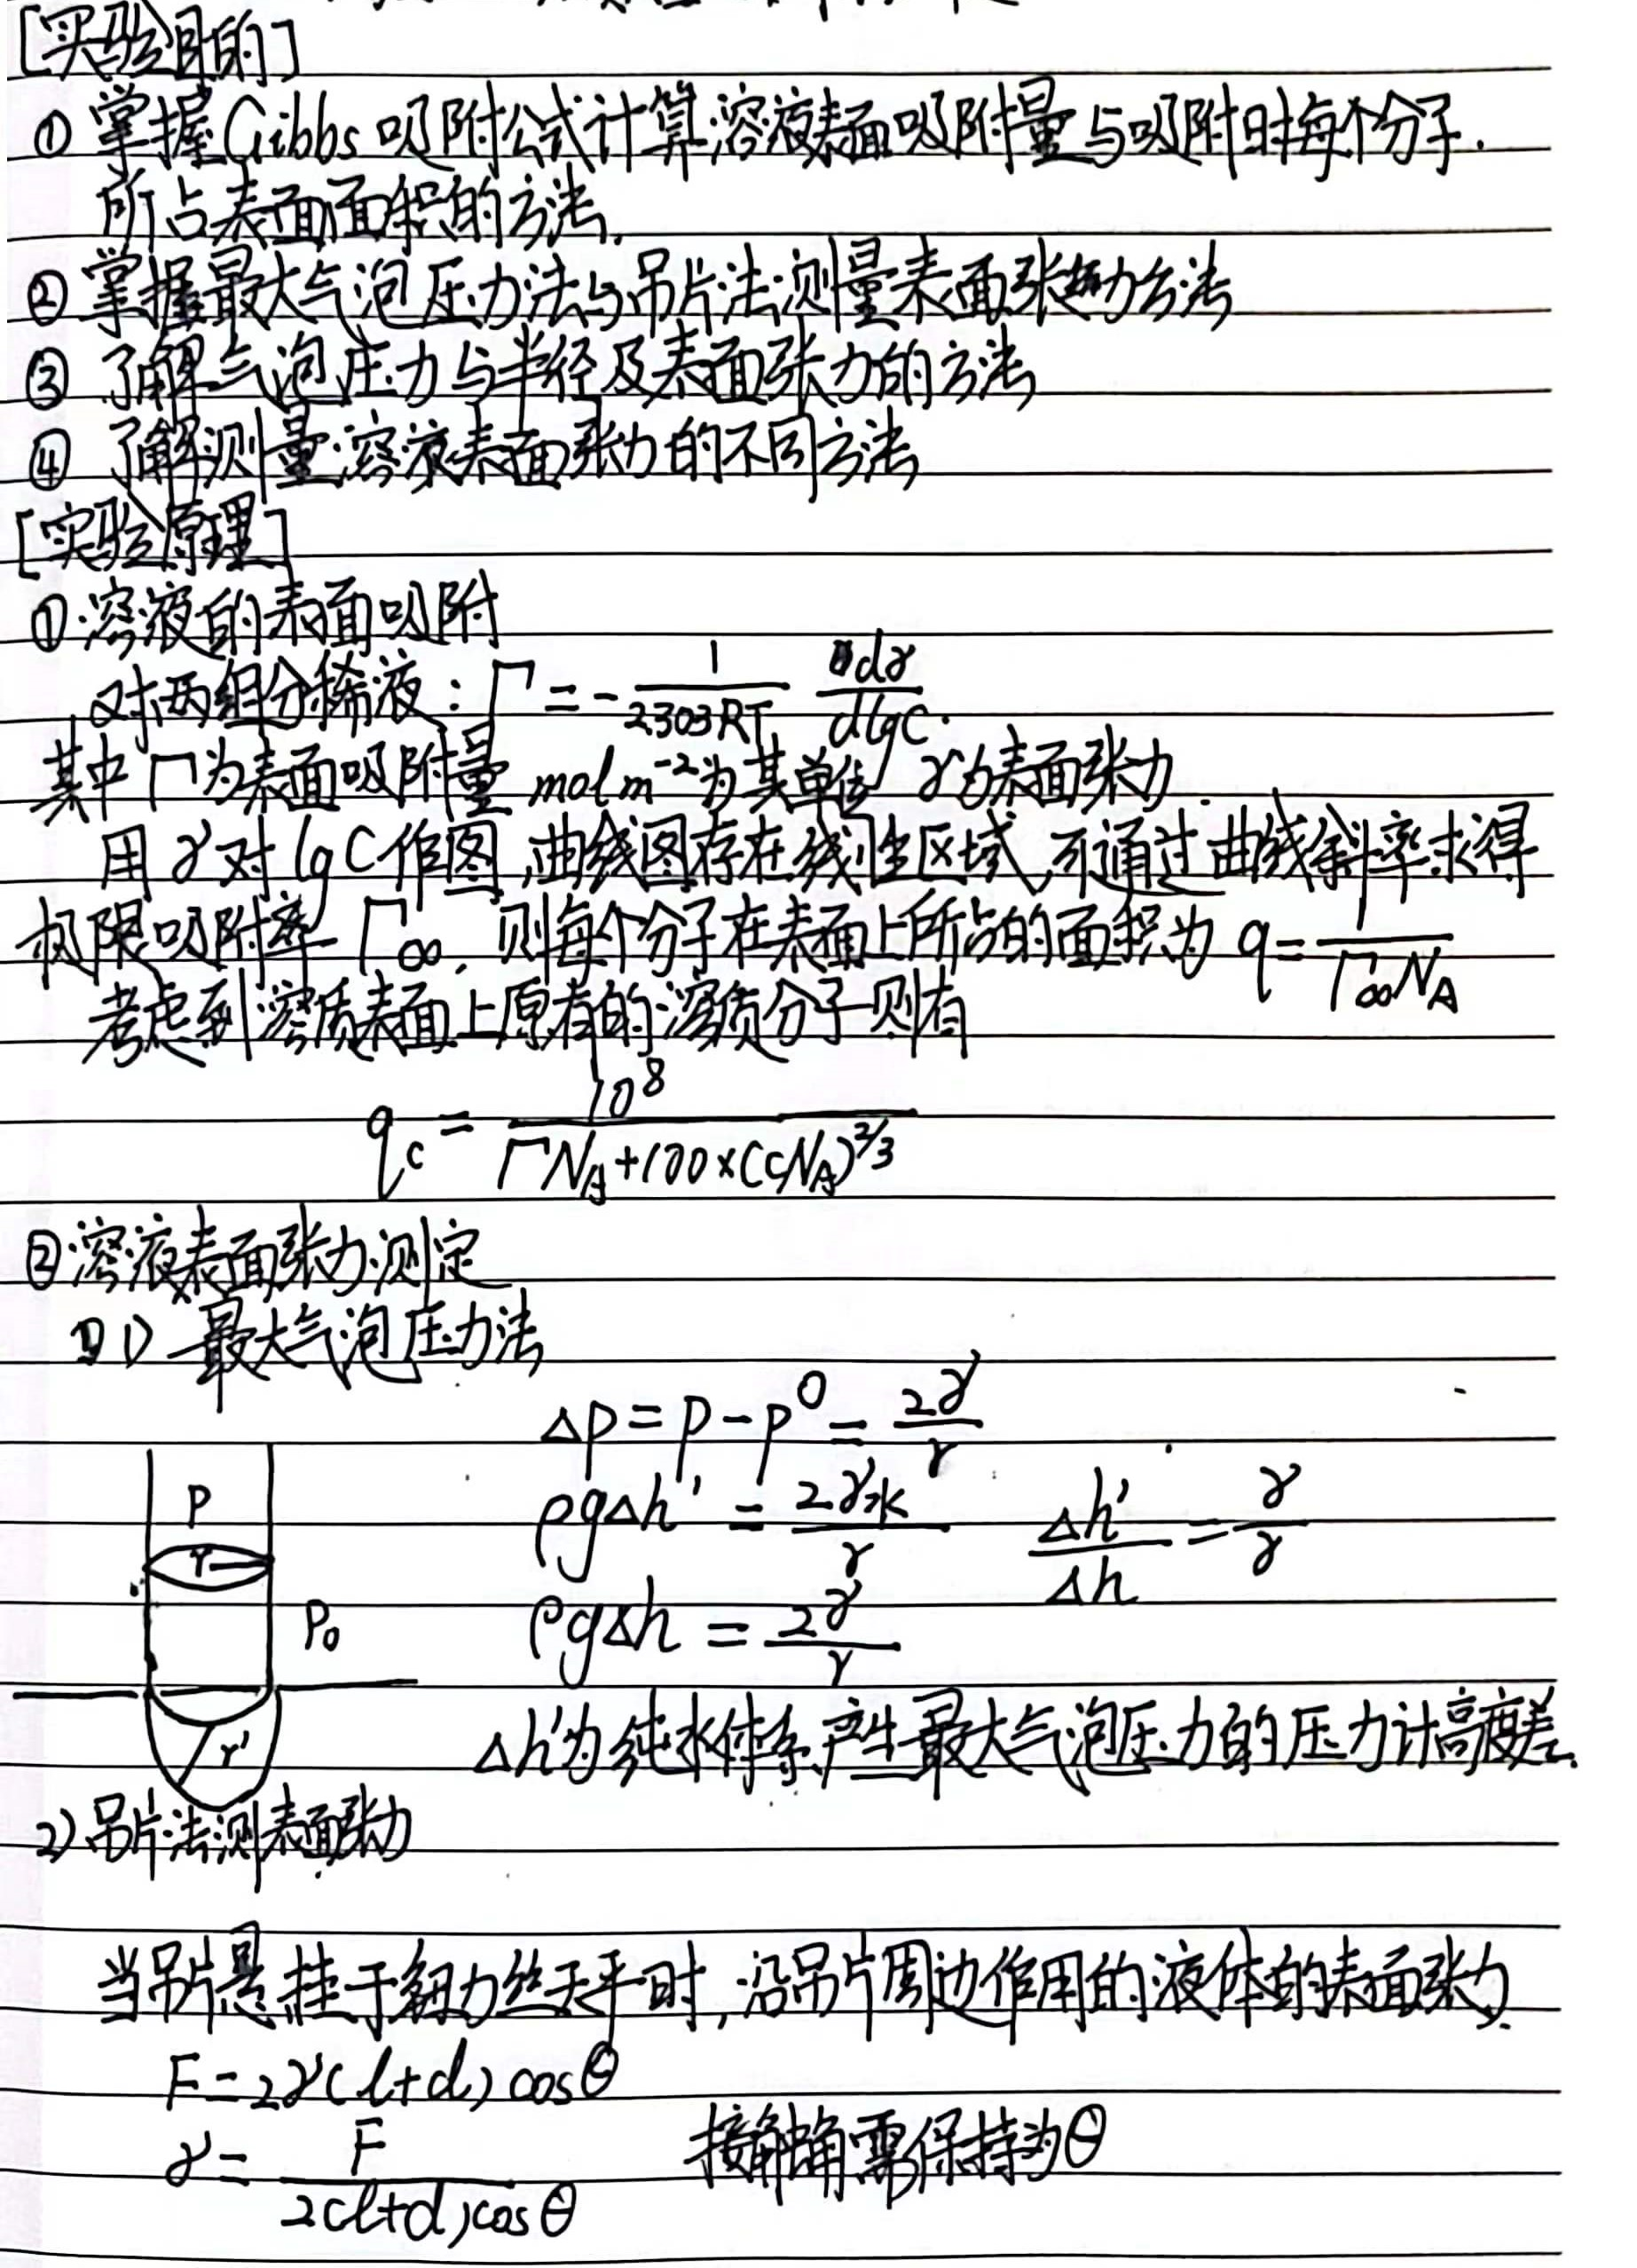
\includegraphics[width = .70\textwidth]{image/yxbg_1.jpg}
    \caption{实验的目的、原理}\label{1}
\end{figure}

\subsection{实验方法}

用最大气泡压力法与吊片法测定表面张力。

\section{实验部分}

\subsection{实验步骤}

实验步骤详见预习报告图~\ref{b} 与图~\ref{4} 。
\begin{figure}[htbp]
    \centering
    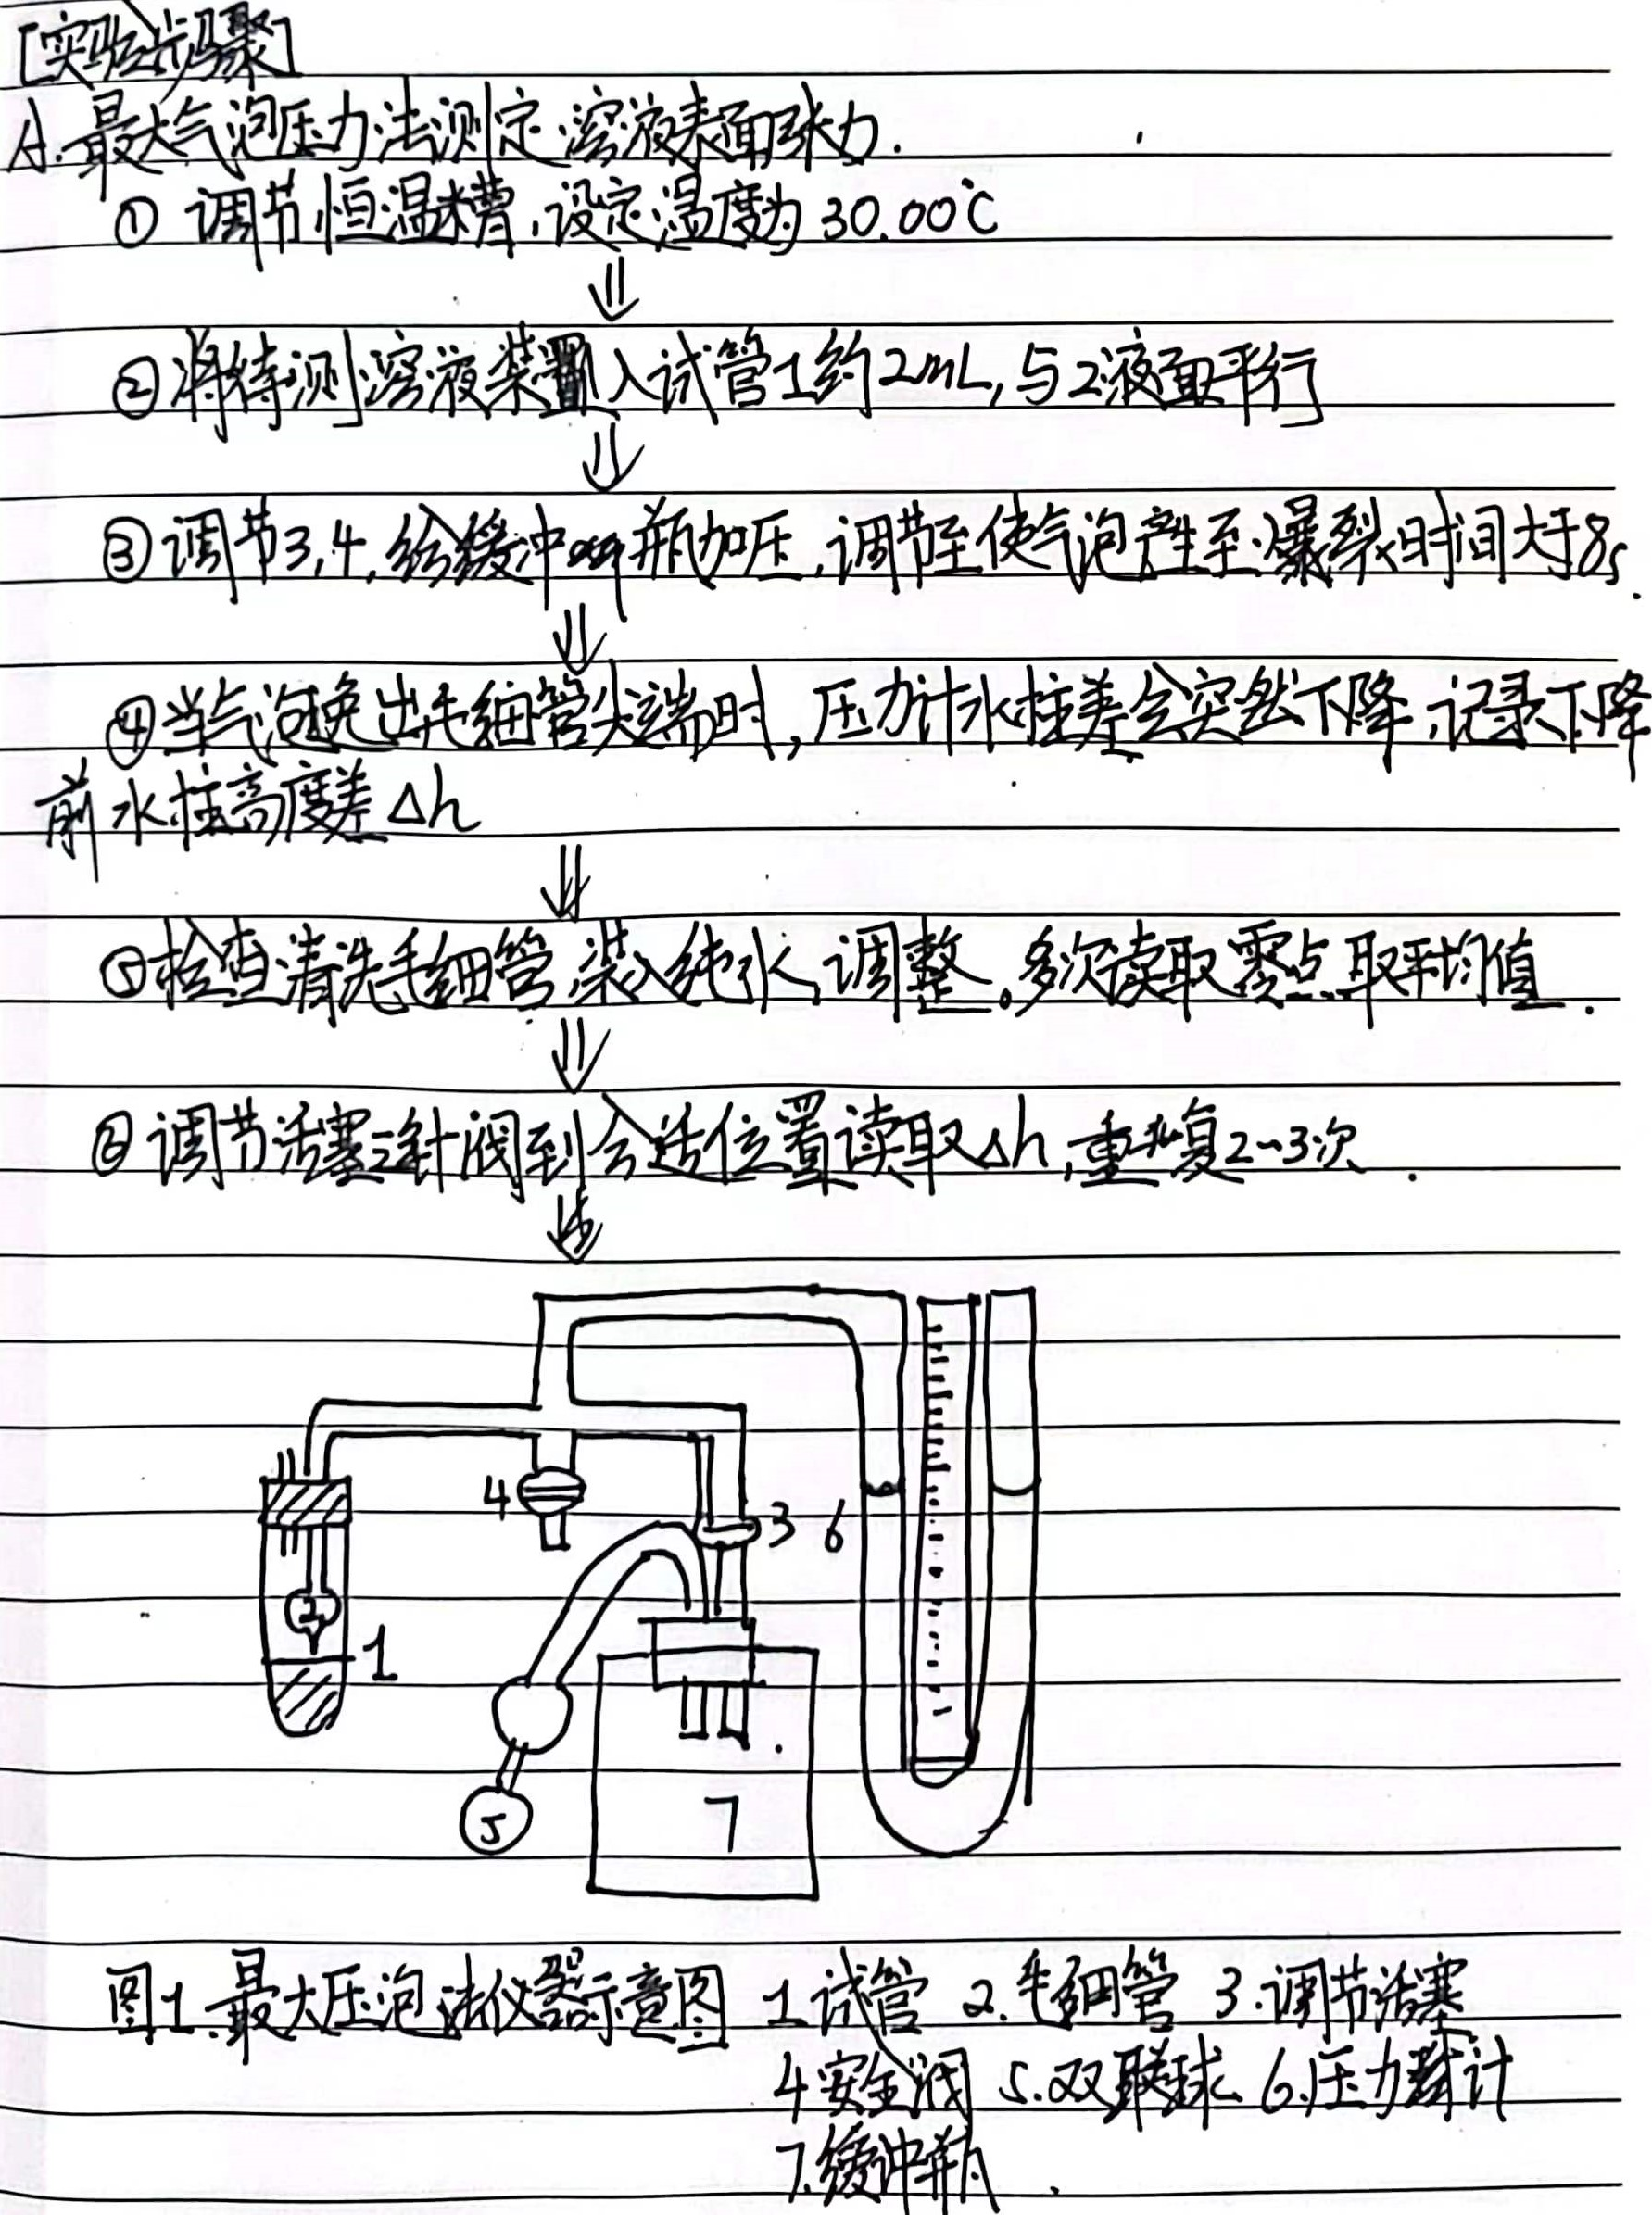
\includegraphics[width = .70\textwidth]{image/yxbg_2.jpg}
    \caption{实验步骤}\label{b}
\end{figure}

\begin{figure}[htbp]
    \centering
    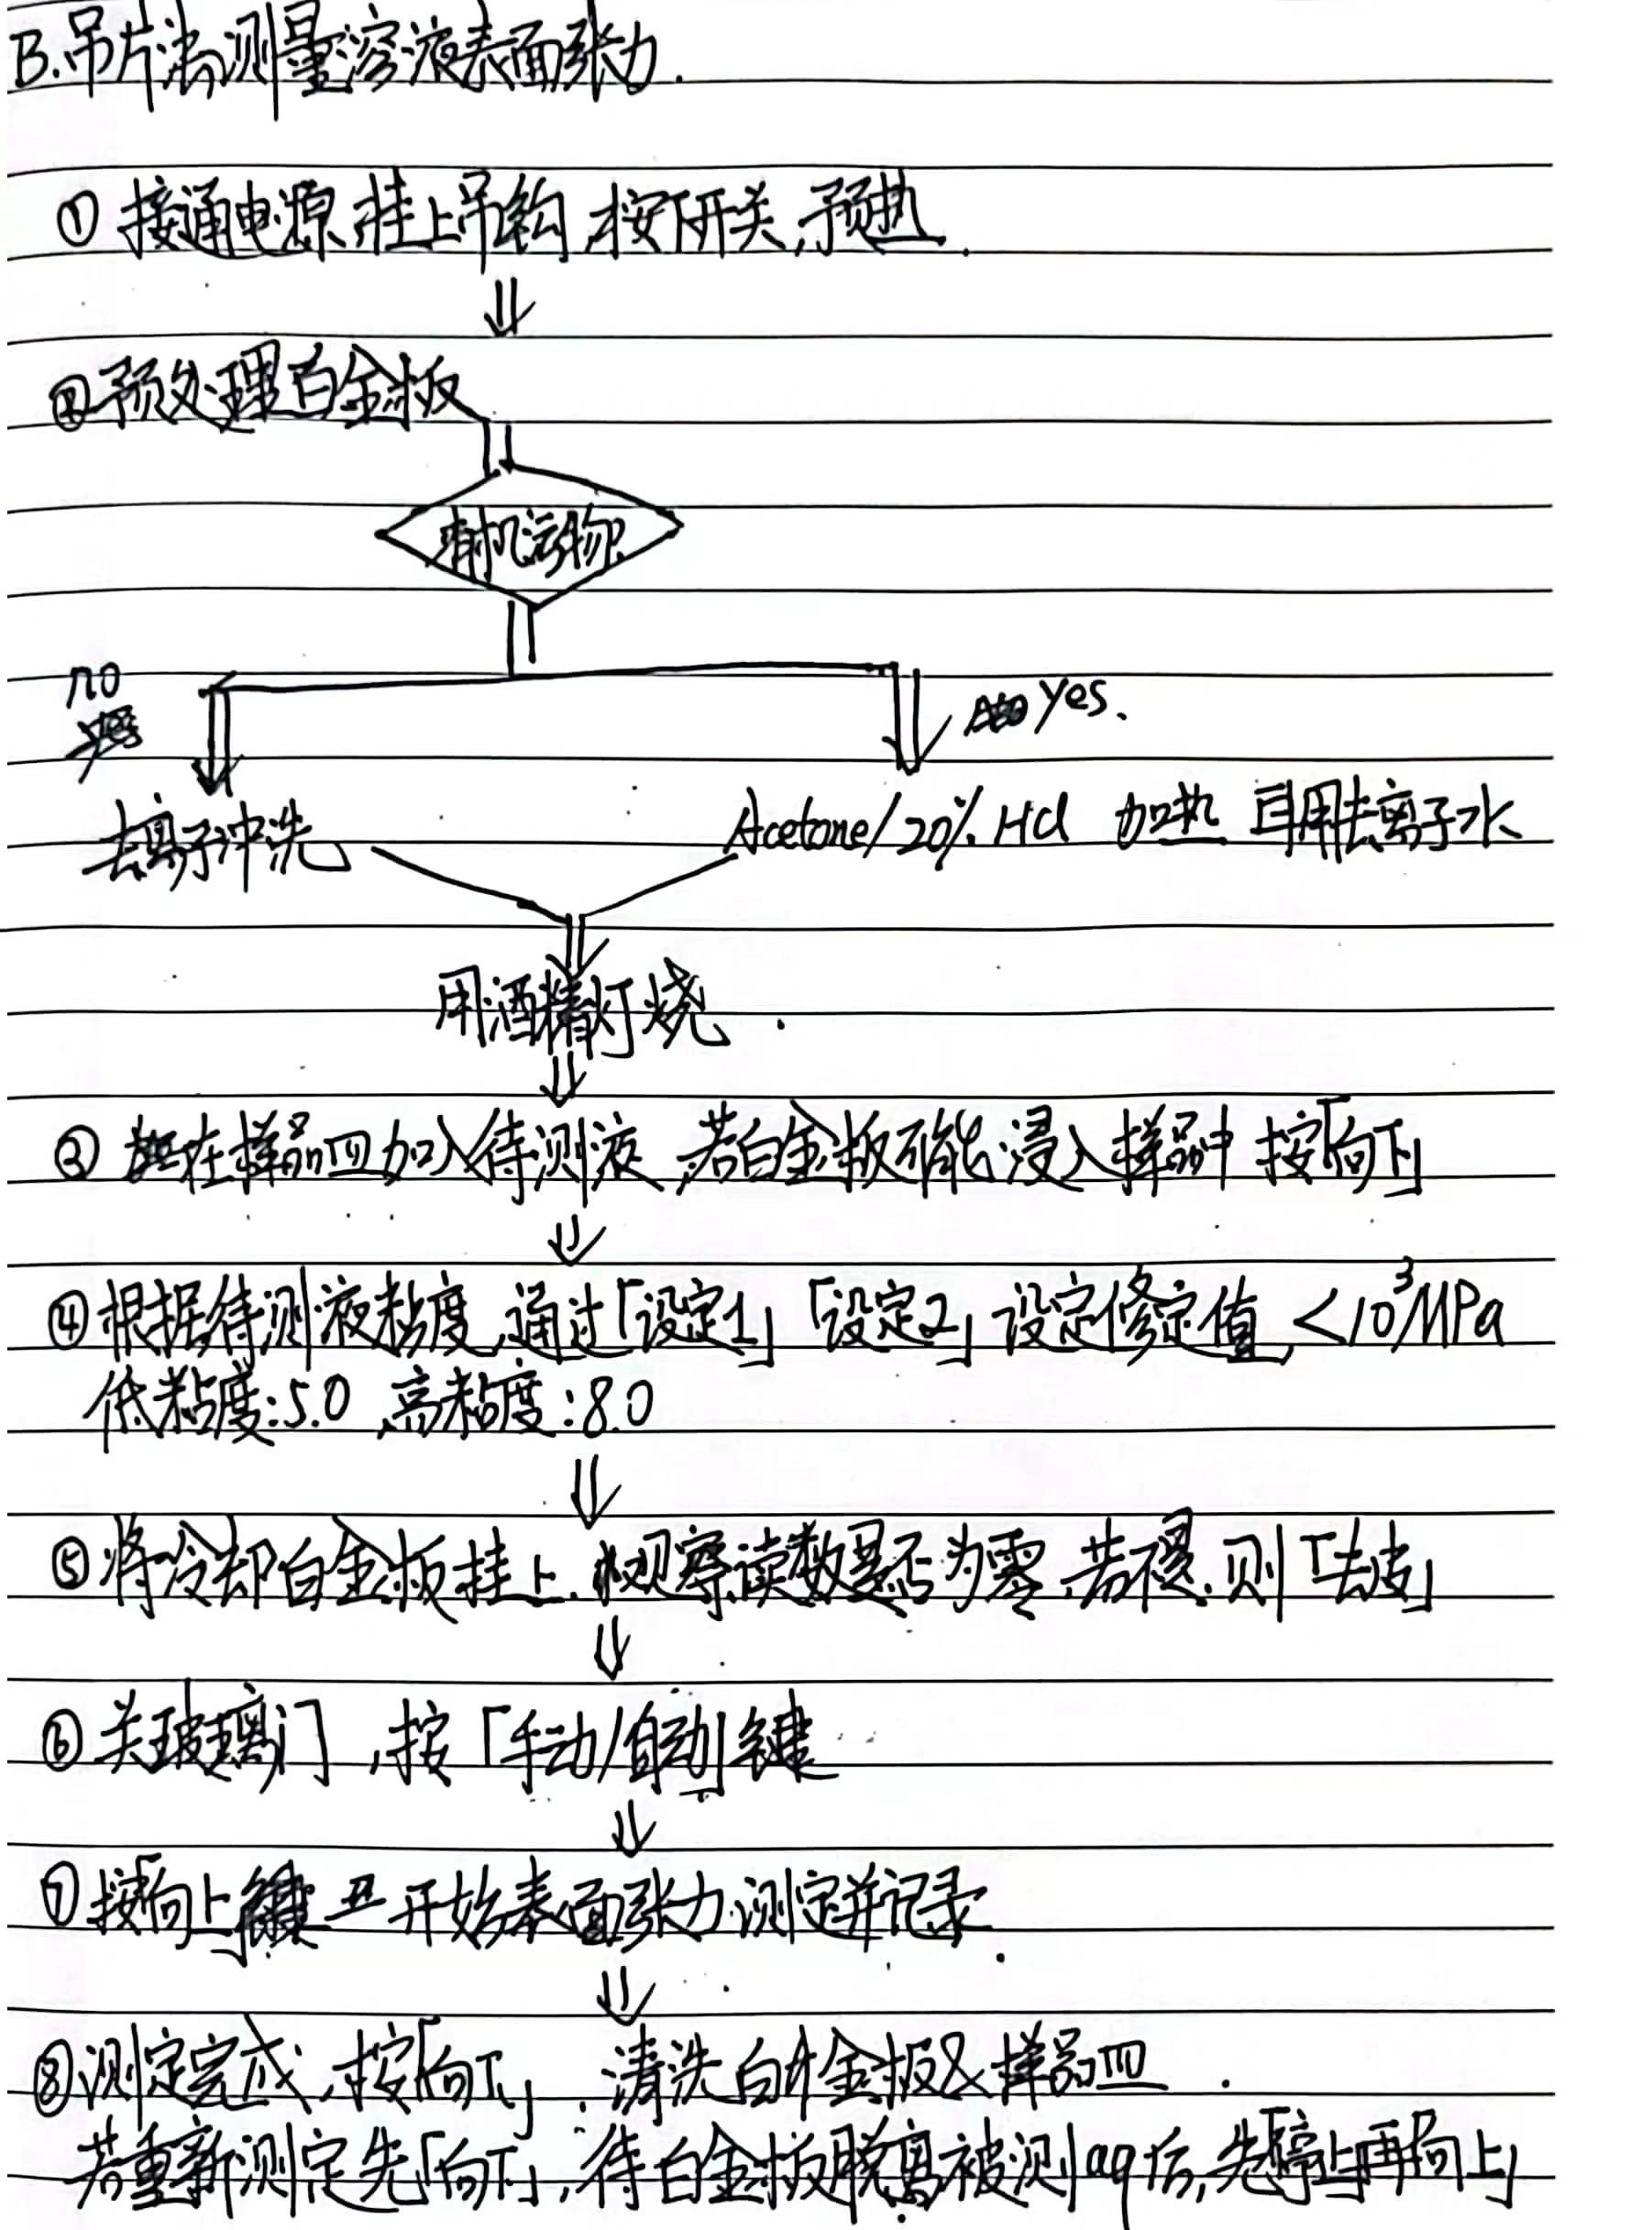
\includegraphics[width = .70\textwidth]{image/yxbg_3.jpg}
    \caption{实验步骤(续)}\label{4}
\end{figure}

\newpage

\subsection{仪器与药品}

\begin{enumerate} %有序列表
    \item 试剂 \\不同浓度的正丁醇溶液(0.0218 mol/L,0.0547 mol/L,0.111 mol/L,0.220 mol/L,
    0.329 mol/L,0.439 mol/L,0.550 mol/L,0.740 mol/L)。
    \item 仪器 \\ 最大气泡压力法表面张力测量装置,QBZY-2 型表面张力仪。
\end{enumerate}

\section{实验现象与数据处理}

\subsection{最大气泡压力法}

    清洗毛细管和试管,装入去离子水。将装置与大气压联通,恒定装置温度为30 ℃,读取零点位置为
$$
    h_0 =\ 22.73 cm 
$$

关闭阀门,调节活塞3的针阀位置至合适位置,读取气泡破裂前最大压力计高度三次。更换溶液重复上述操作,记录浓度与
压力计高度读数平均值,并计算左右压力计高度差如下表 \ref{5} 。

\begin{table}[h]
    \centering
    \caption{最大气泡压力法的测量结果}
    \label{5}
    \begin{tabular}{cccccc}
    \hline
    c/$\rm   mol \cdot L^{-1}$ & $\ln c$ & $\rm h_{left} / cm$ & $\rm h_{right} / cm$ & $\rm \Delta h / cm$ & $\gamma / {\rm mN \cdot m^{-1}}$ \\ \hline
    0.00   &   --  & 18.00 & 27.49 & 9.49 & 71.18 \\
    0.0218 & -3.83 & 18.39 & 27.05 & 8.66 & 64.95 \\
    0.0547 & -2.91 & 18.82 & 26.65 & 7.83 & 58.73 \\
    0.111  & -2.20 & 19.23 & 26.19 & 6.96 & 52.20 \\
    0.220  & -1.51 & 19.80 & 25.63 & 5.83 & 43.73 \\
    0.329  & -1.11 & 20.17 & 25.28 & 5.11 & 38.33 \\
    0.439  & -0.82 & 20.48 & 25.03 & 4.55 & 34.13 \\
    0.550  & -0.60 & 20.60 & 24.85 & 4.25 & 31.88 \\
    0.740  & -0.30 & 20.91 & 24.55 & 3.64 & 27.30 \\ \hline
    \end{tabular}
\end{table}


由于在最大气泡压力法中
$$
    \Delta {\rm P} = \rho g \Delta h = 2 \gamma / r
$$

因此,查表可知,纯水的表面张力为 $ 71.18\ mN \cdot m^{-1}$。 可以通过
$$
    \gamma = \gamma_{H_2O} \cdot \frac{\Delta h}{\Delta h_{H_2O}}
$$

计算得到不同浓度下的表面张力。

\subsection{吊片法}

使用表面张力仪测量纯水和不同浓度正丁醇溶液的表面张力,如表 \ref{6} 所示。

\begin{table}[h]
    \centering
    \caption{吊片法的测量结果}
    \label{6}
    \begin{tabular}{ccc}
    \hline
    c/$\rm   mol \cdot L^{-1}$ & $\ln c$ & $\gamma / {\rm mN \cdot m^{-1}}$ \\ \hline
    0.00                       & --      & 71.00                            \\
    0.0218                     & -3.83   & 30.43                            \\
    0.0547                     & -2.91   & 34.12                            \\
    0.111                      & -2.20   & 36.77                            \\
    0.220                      & -1.51   & 40.56                            \\
    0.329                      & -1.11   & 45.84                            \\
    0.439                      & -0.82   & 53.94                            \\
    0.550                      & -0.60   & 60.87                            \\
    0.740                      & -0.30   & 66.50                            \\ \hline
    \end{tabular}
\end{table}

本次实验的吊片法为本组成员共同完成,每人负责测定 1 - 2 组数据。测量温度取室温 21℃

\subsection{水的饱和吸附量的计算}

使用最大气泡压力法,用表 \ref{5} 的数据将 $\gamma$ 对 $\ln c$ 作图,如图 \ref{7},并对高浓度的线性部分做线性回归
回归结果为 
$$
\gamma = 23.424 \pm 0.341 + ( - 13.395 \pm 0.354) \cdot \ln c
\quad R^2 = 0.9972
$$



由公式
$$
    \varGamma_\infty = - \frac{1}{RT} \frac{d \gamma}{d \ln c}
$$

且
$$
    \frac{d \gamma}{d \ln c} = - 13.395
$$

可得
$$
    \varGamma_\infty = - \frac{ - 13.395 \cdot 10^{-3} }{8.314 \cdot 303.15 } {\rm\ mol \cdot m^{-2}} = 5.3 \cdot 10^{-6} {\rm\ mol \cdot m^{-2}}
$$

\begin{figure}[h]
    \centering
    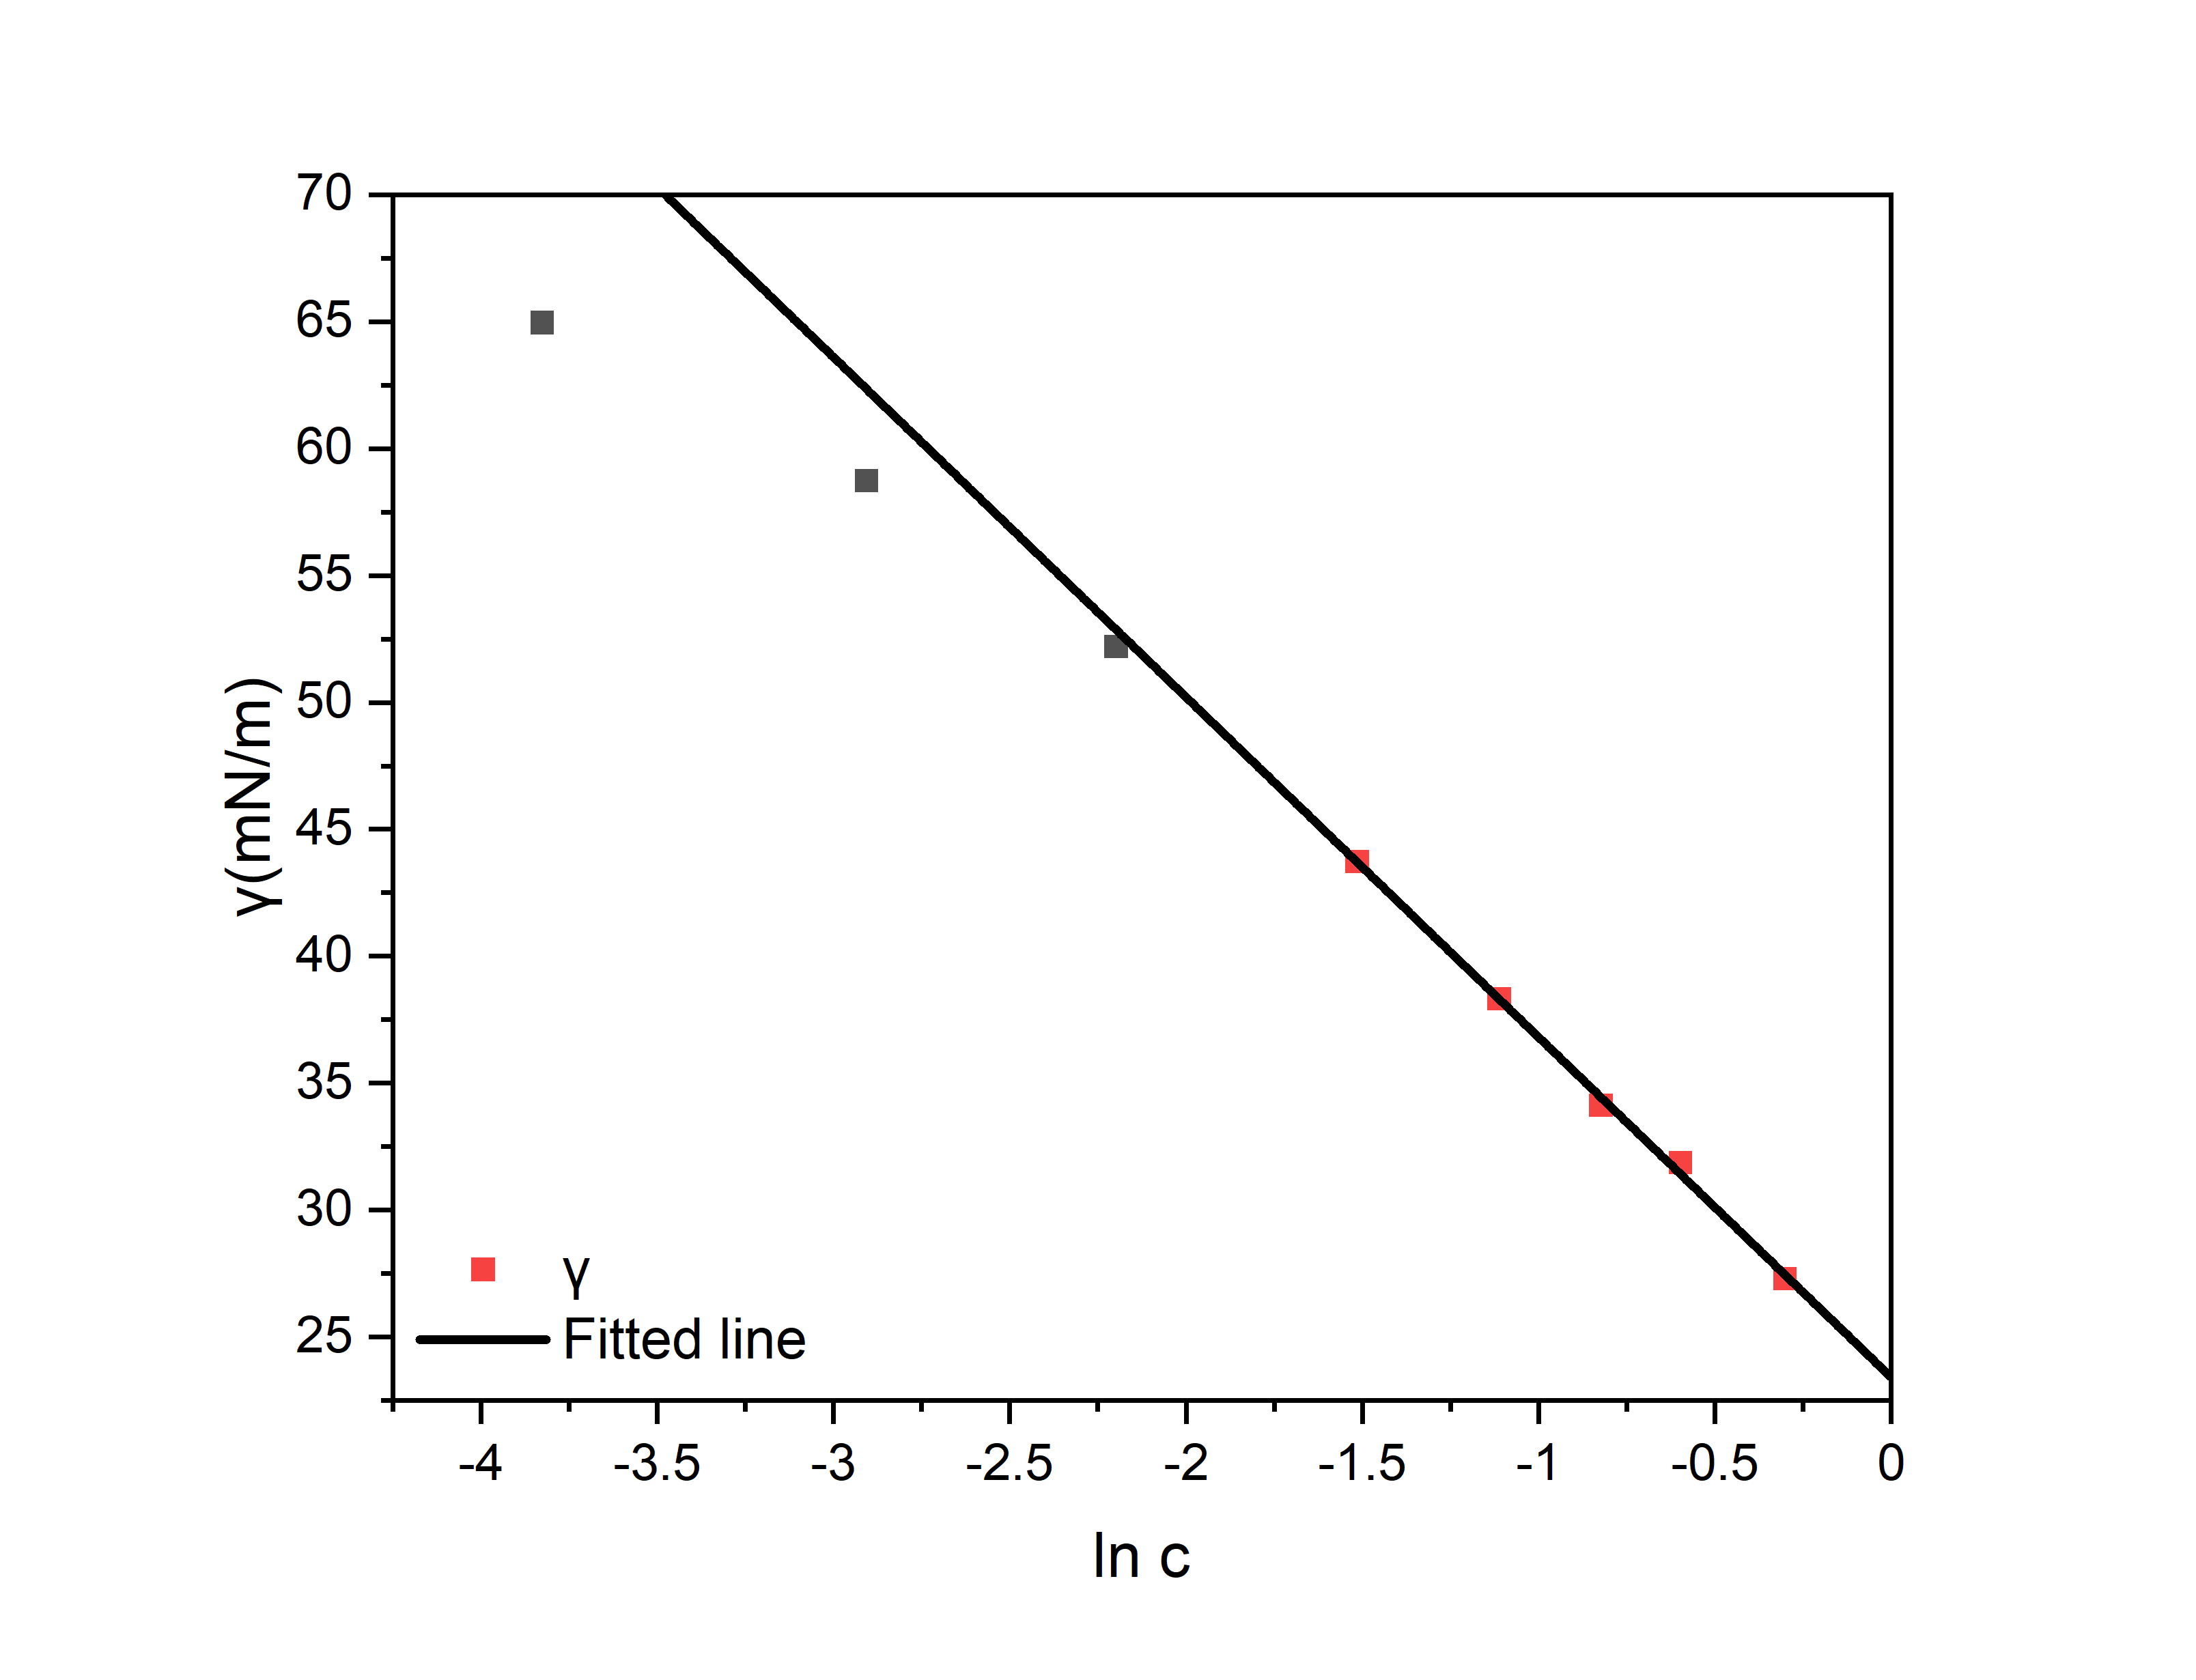
\includegraphics[width = .65\textwidth]{image/Graph2.png}
    \caption{最大气泡压力法的$\gamma - \ln c$图}\label{7}
\end{figure}

对其进行误差分析

\begin{equation*}
    \begin{split}
    \rm \sigma_{\varGamma_\infty} 
    &= \sqrt{(\frac{1}{RT} \cdot \sigma_T)^2 + (\frac{1}{RT} \cdot \sigma_
    {\frac{d \gamma}{d \ln c}})^2} \\
    &= \sqrt{(\frac{1}{8.314 \cdot 303.15} \cdot \frac{0.01}{303.15})^2 + (\frac{1}{8.314 \cdot 303.15} \cdot 0.354 \cdot 10^{-3})^2}
    \\
    &= 1.41 \cdot 10^{-7}   
    \end{split}
\end{equation*}

因此最大气泡压力法饱和吸附量为 $(5.3 \pm 0.1) \cdot 10^{-6} {\rm\ mol \cdot m^{-2}}$。

使用同样的处理步骤对吊片法数据作 $\gamma - \ln c$图如图 \ref{8} 所示。线性回归结果为
$$
\gamma = 26.502 \pm 0.148 + ( - 12.698 \pm 0.154) \cdot \ln c
\quad R^2 = 0.9996
$$

\begin{figure}[h]
    \centering
    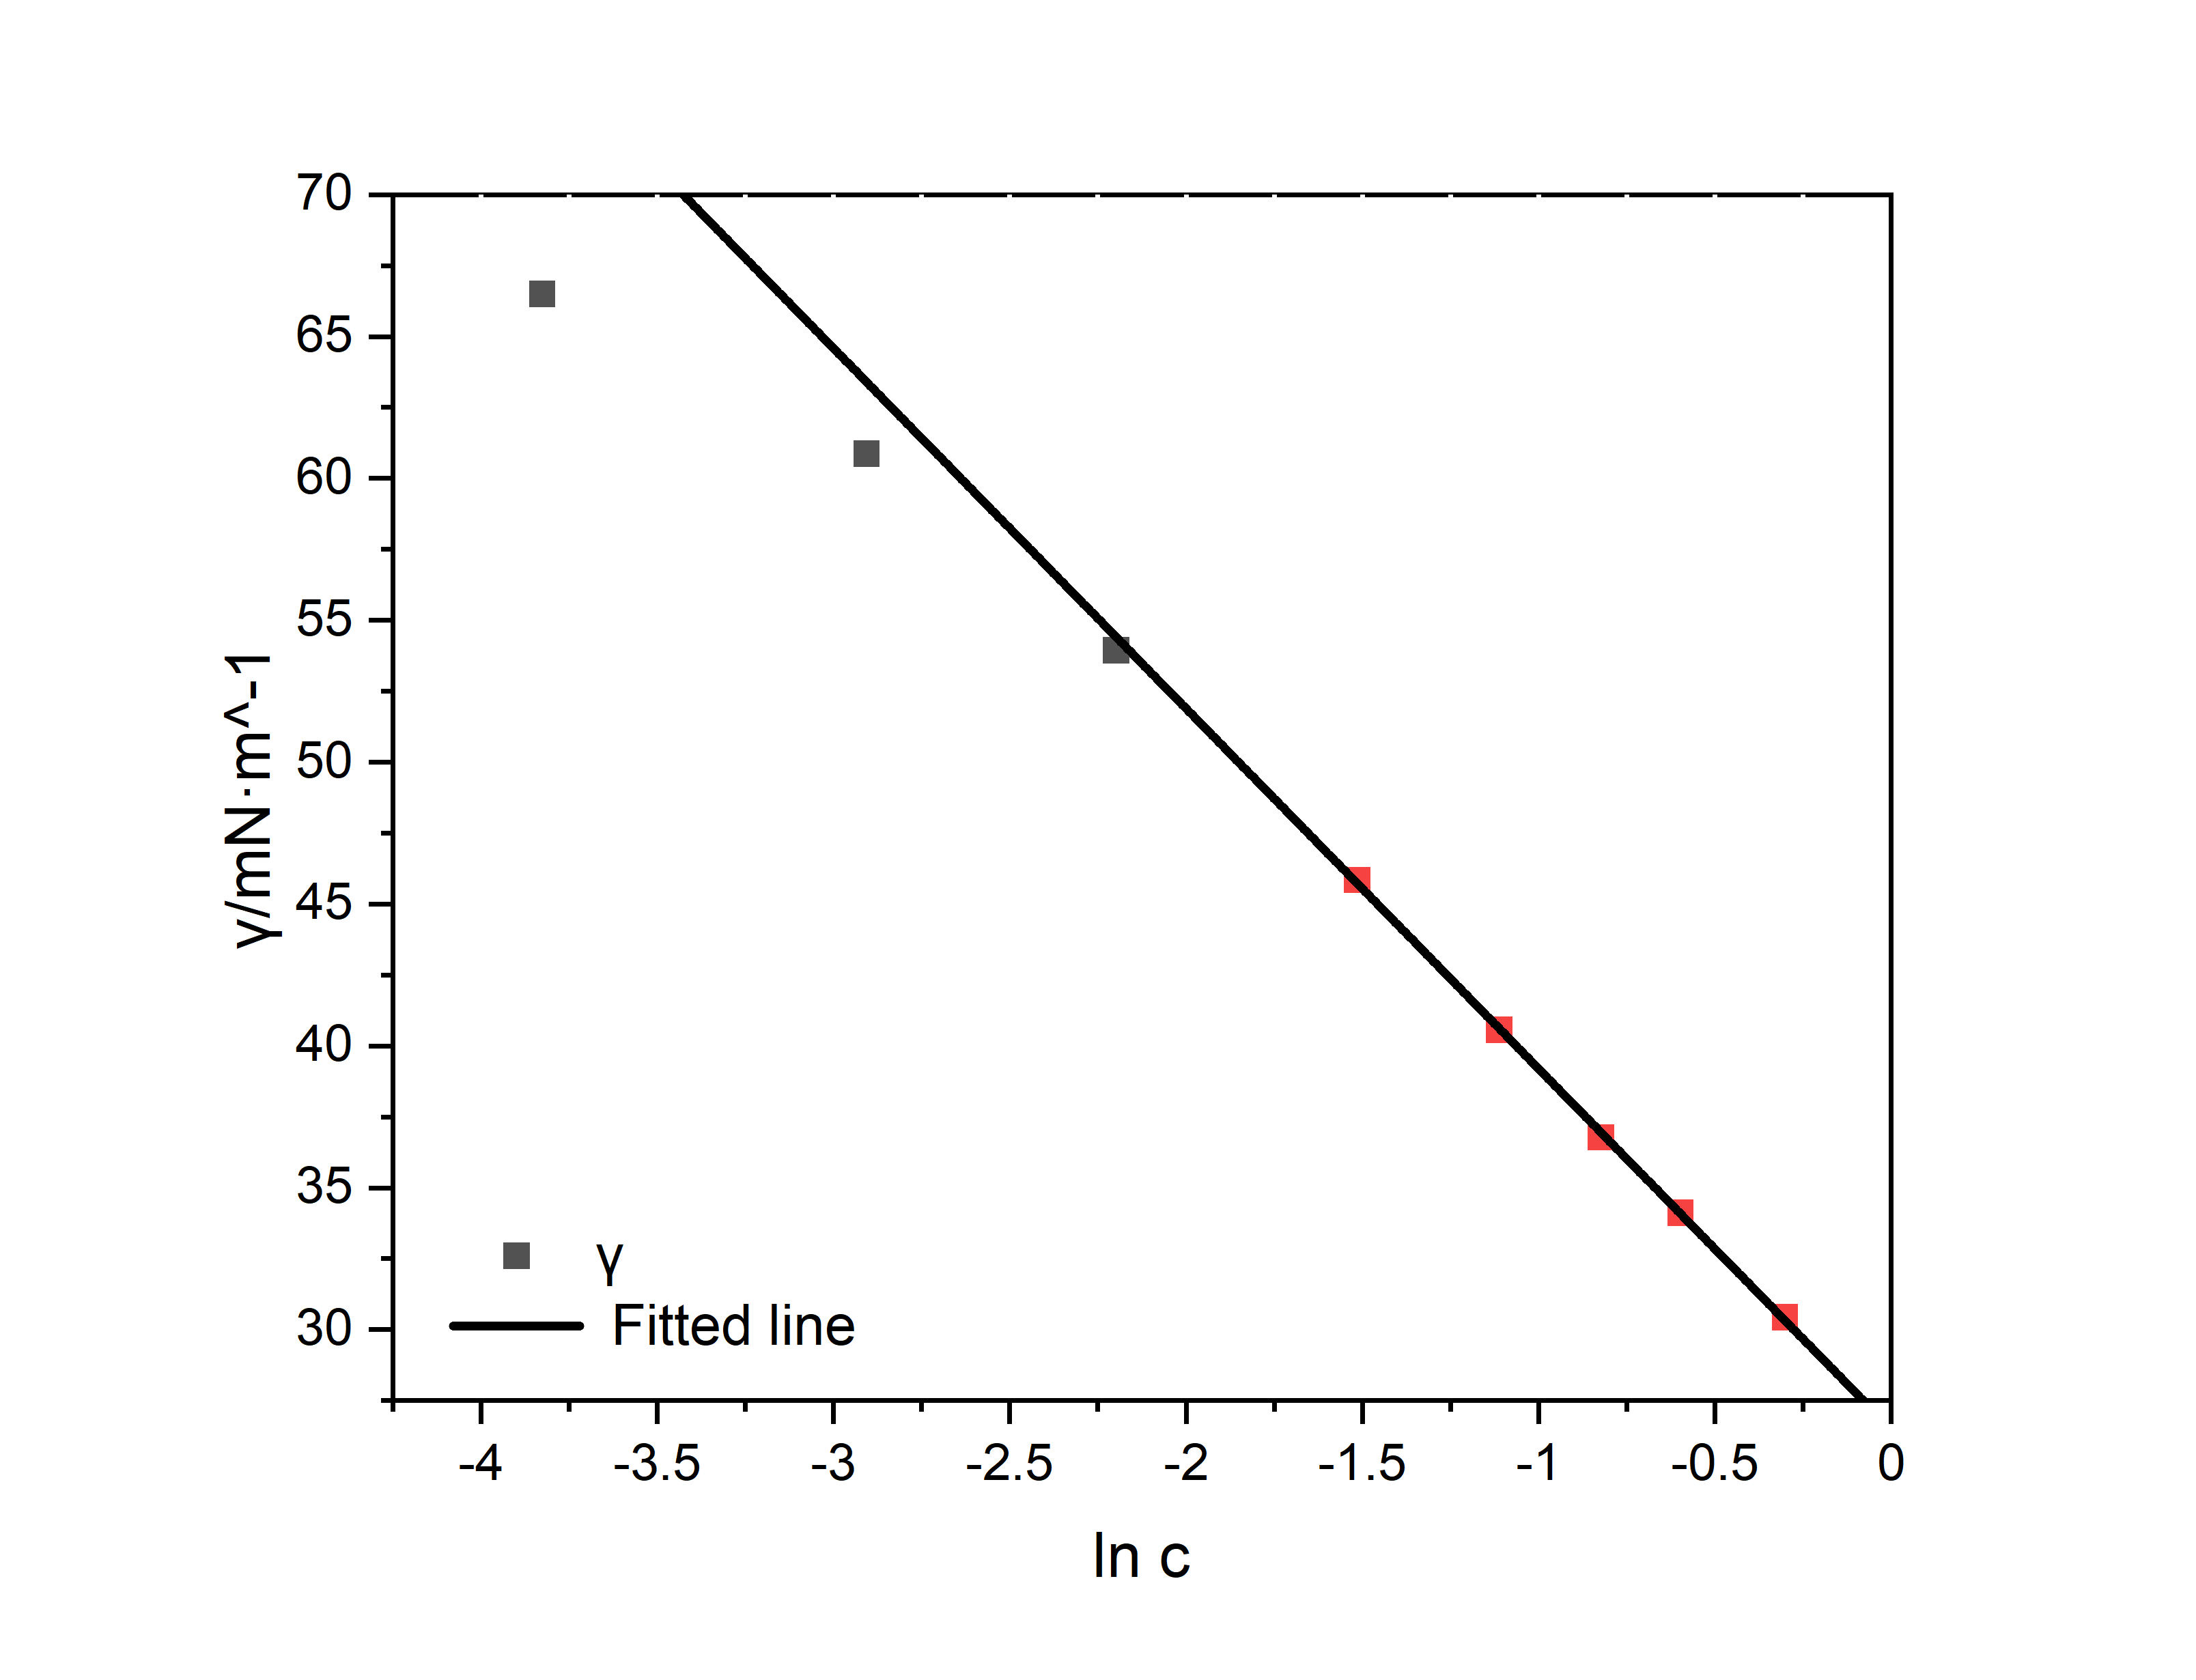
\includegraphics[width = .65\textwidth]{image/Graph4.png}
    \caption{吊片法$\gamma - \ln c$图}\label{8}
\end{figure}

处理可得
$$
    \varGamma_\infty = - \frac{ -  12.698  \cdot 10^{-3} }{8.314 \cdot 294.15 } {\rm\ mol \cdot m^{-2}} = 5.19 \cdot 10^{-6} {\rm\ mol \cdot m^{-2}}
$$

对其进行误差分析
\begin{equation*}
    \begin{split}
    \rm \sigma_{\varGamma_\infty} 
    &= \sqrt{(\frac{1}{RT} \cdot \sigma_T)^2 + (\frac{1}{RT} \cdot \sigma_
    {\frac{d \gamma}{d \ln c}})^2} \\
    &= \sqrt{(\frac{1}{8.314 \cdot 303.15} \cdot \frac{0.01}{303.15})^2 + (\frac{1}{8.314 \cdot 303.15} \cdot 0.154 \cdot 10^{-3})^2}
    \\
    &= 6.25 \cdot 10^{-8}
    \end{split}
\end{equation*}

因此吊片法饱和吸附量为 $(5.19 \pm 0.06) \cdot 10^{-6} {\rm\ mol \cdot m^{-2}}$

可以看出使用最大气泡压力法的误差稍高于吊片法,
最大气泡压力法可能带来误差的原因是压力计的读数存在误差,
并且不同浓度溶液控制气泡冒出的时间有所不同,随着正丁醇浓度增大,其气泡越来越稳定,可能会不破裂并积蓄在液面上,也会对读数造成影响。
此外,毛细管插入深度的差异也会对测量的压力带来误差。
由于吊片法仪器给出的是一段表面张力的范围,吊片法的误差来源可能为不同人的读数选取存在差异,样品皿没有完全清洗干净等。


\subsection{表面吸附分子的横截面积}

使用最大气泡压力法,若不考虑表面原有的溶质分子,由公式可得表面吸附分子的横截面积为
$$
   q = \frac{1}{N_A \varGamma_\infty} = \frac{1}{5.3 \cdot 10^{-6} \cdot  6.023 \cdot 10^{23}} = 3.1 \cdot 10^{-19}{\rm\ m^2} = 0.31{\rm\ nm^2}
$$

其误差分析方法为
$$
\rm \sigma_{q} = \sqrt{(\frac{\sigma_{\varGamma_\infty}}{\varGamma_\infty^2 N_A} )^2} = \frac{1.41 \cdot 10^{-7} }{(5.3 \cdot 10^{-6})^2 \cdot  6.023 \cdot 10^{23}} = 8.33 \cdot 10^{-21}\ m^2 = 0.00833\ nm^2
$$

因此若不考虑表面溶质分子,最大气泡压力法表面吸附分子的横截面积为 $0.31 \pm 0.01 {\rm\ nm^{-2}}$。

当溶液浓度较高,表面会存在原有溶质分子,此时由如下公式溶液表面吸附分子的横截面积

$$
   q_c = \frac{1}{N_A \varGamma + (cN_A)^{2/3}} 
$$

其误差分析公式为
$$
\rm \sigma_{q_c} = \sqrt{(\frac{\sigma_{\varGamma_\infty} N_A}{(\varGamma_\infty N_A + (cN_A)^{2/3})^2} )^2+(\frac{2}{3} \cdot \frac{c^{-1/3}N_A^{2/3}\sigma_c}{(\varGamma_\infty N_A+(cN_A)^{2/3})^2})^2} 
$$

对各组数据使用如上公式计算。结果如表 \ref{9} 。
\begin{table}[h]
    \centering
    \caption{最大气泡压力法高浓度下的饱和吸附分子横截面积}
    \label{9}
    \begin{tabular}{ccc}
    \hline
    c/$\rm   mol \cdot L^{-1}$ & $q_c/{\rm nm^2}$ & $\sigma_{q_c}/{ \rm nm^2}$ \\ \hline
    0.220                      & 0.308 & 0.008    \\
    0.329                      & 0.306 & 0.008    \\
    0.439                      & 0.305 & 0.008    \\
    0.550                      & 0.303 & 0.008    \\
    0.740                      & 0.301 & 0.008    \\ \hline
    \end{tabular}
\end{table}


使用吊片法,使用同样的公式计算溶液表面吸附分子的横截面积
$$
   q = \frac{1}{N_A \varGamma_\infty} = \frac{1}{5.19 \cdot 10^{-6} \cdot  6.023 \cdot 10^{23}} = 3.20 \cdot 10^{-19}{\rm\ m^2} = 0.320{\rm\ nm^2}
$$

对其进行误差分析
$$
\rm \sigma_{q} = \sqrt{(\frac{\sigma_{\varGamma_\infty}}{\varGamma_\infty^2 N_A} )^2} = \frac{1.41 \cdot 10^{-7} }{(5.3 \cdot 10^{-6})^2 \cdot  6.023 \cdot 10^{23}} = 3.85 \cdot 10^{-21}\ m^2 = 0.00385\ nm^2
$$

因此吊片法表面吸附分子的横截面积为 $0.320 \pm 0.004 {\rm\ nm^{2}}$。

同样地,考虑溶质分子的影响,不同浓度下饱和吸附分子横截面积如下表 \ref{10} 所示。
\begin{table}[h]
    \centering
    \caption{吊片法高浓度下的饱和吸附分子横截面积}
    \label{10}
    \begin{tabular}{ccc}
    \hline
    c/$\rm   mol \cdot L^{-1}$ & $q_c/{\rm nm^2}$ & $\sigma_{q_c}/{\rm nm^2}$ \\ \hline
    0.220                      & 0.314 & 0.004          \\
    0.329                      & 0.313 & 0.004          \\
    0.439                      & 0.311 & 0.004          \\
    0.550                      & 0.310 & 0.004          \\
    0.740                      & 0.308 & 0.004          \\ \hline
    \end{tabular}
\end{table}

对比忽略分子影响与考虑溶质分子的数据,可以发现在高浓度下,溶质分子的参与会对数据造成较大的偏离,因此在浓度较高时应当考虑溶质分子的影响。



\section{实验结果与讨论}

\subsection{结论}

本次实验使用最大气泡压力法与吊片法,测量了纯水以及不同浓度的正丁醇溶液的表面张力大小
并通过实验数据,作 $\gamma-\ln c$ 图来计算 $d \gamma / d \ln c$ ,从而求得水的饱和吸附量,并对计算进行误差分析。
得到最大气泡压力法饱和吸附量为 $(5.3 \pm 0.1) \cdot 10^{-6} {\rm\ mol \cdot m^{-2}}$
,吊片法饱和吸附量为 $(5.19 \pm 0.06) \cdot 10^{-6} {\rm\ mol \cdot m^{-2}}$。
最后,再计算两种方法下吸附分子的横截面积。其中最大气泡压力法表面吸附分子的横截面积为 $0.31 \pm 0.01 {\rm\ nm^{-2}}$,
吊片法表面吸附分子的横截面积为 $0.320 \pm 0.004 {\rm\ nm^{2}}$,并计算了高浓度下考虑溶质分子的横截面积$q_c$。

\nocite{*}
\bibliography{reference}
\end{document}
